\documentclass[fleqn]{MJD}

\usepackage{cancel}
\usepackage{cleveref}
\usepackage{titlesec}
\usepackage{hyperref}
%\colorsections
%\bluelinks
\newcommand{\problem}[1]{\chapter{Problem #1}}
\newcommand{\subproblem}[2]{\section{(#1)~ #2}}
\newcommand{\subsubproblem}[2]{\subsection{ #1)~ #2}}
\newcommand{\U}{\cup}
\renewcommand{\S}{\mathcal{S}}
\renewcommand{\s}{\subset}
\renewcommand{\equiv}{\Leftrightarrow}
\newcommand{\0}{\emptyset}
\newcommand{\imp}{\Rightarrow}
\newcommand{\Usum}{\bigcup\limits_{i=1}^\infty}
\newcommand{\intsum}{\bigcup\limits_{i=1}^\infty}
\newcommand{\infsum}{\sum\limits_{i=1}^\infty}
\newcommand{\sets}{\{A_1, A_2 \dots\} }
\newcommand{\nsets}{\{A_1, \dots, A_n \} }

\titleformat{\chapter}[display]
  {\normalfont\bfseries}{}{0pt}{\LARGE}
  
\graphicspath{ {../} }

%%%%%%%%%%%%%%%%%%%%%%%%%%%%%%%%%%%%
\begin{document}
\lstset{language=Python}
\titleAT[CS 224N: Assignment 3]{Peter888@stanford.edu}
%-------------------------------------
\problem{1. A window into NER (30 points)}
%-------------------------------------

%----------------------
\subproblem{a}{ Understanding NER (5 points, written)}
\subsubproblem{i} {Ambiguous Examples (2 points)} 
\noindent\textbf{Answer:} \\
\indent 1. "Walt Disney has just bought Fox for 52bn", here "Walt Disney" and "Fox" are ambiguous type. "Walt Disney" can stands for person, the founder of Walt Disney Company, or can stands for "Walt Disney" organization, the company. \\
\indent 2. "What does the Fox say", here "Fox" is ambiguous type. "Fox" can stands for the animal, or can stands for "Fox" organization, the company.
\subsubproblem{ii} {Why use features (1 point)} 
\noindent\textbf{Answer: } \\
\indent Words can have multiple means depending on it's context. We need predict named entity labels from their context as well. \\
\subsubproblem{iii} { Feature examples (2 points)} 
\noindent\textbf{Answer:} \\
\indent 1. Adjacent Verb. For example "Rose said", here Rose should be a person, not the flower rose, because it's adjacent verb "said" \\ 
\indent 2. Location. If "Chase" happening on highway, that's normally the verb chase, instead of the bank "Chase"
\vskip3em

%----------------------
\subproblem{b}{ Computational complexity (5 points, written)}
\subsubproblem{i} {Dimensions (2 points)} 
\noindent\textbf{Answer:} \\
\indent $\bm{e}^{(t)} \in \mathbb{R}^{1 \times ((2\omega + 1)\times D)}$, $\bm{W} \in \mathbb{R}^{(2\omega + 1)\times H}$,  $\bm{U} \in \mathbb{R}^{H \times C}$
\subsubproblem{ii} {Complexity (3 point)} 
\noindent\textbf{Answer:} \\
\indent For each step $\bm{e}^{(t)}$ requires $\bm{O}((2\omega + 1)\times D)$ computation, $\bm{h}^{(t)}$ requires $\bm{O}((2\omega + 1) \times D \times H)$ computation, and $\bm{\hat{y}}^{(t)}$ requires $\bm{O}(H \times C)$ computation. \\
\indent In total, requires $\bm{O}(T \times ((2\omega + 1)\times D + (2\omega + 1) \times D \times H + H \times C))$ computation.  Ignore the constants and $D,H>>C$, the computation complexity of whole sentence is $\bm{O}(T \times \omega \times D \times H)$
\vskip3em
\newpage
%----------------------
\subproblem{c}{Implement model(15 points, code)}
\noindent \textbf{Answer:}  \\ 
See code: $\sim$\verb|/q1_window.py|. \\ And deliverable $\sim$\verb|/window_predictions.conll|
\vskip3em
%----------------------
\subproblem{d}{Analyze the predictions (5 points, written)}
\subsubproblem{i} {Report best $F_{1}$ score (1 point)} 
\indent \textbf{Answer:}  \textit {Get best $F_{1}$ score 0.84. } \\ 
\begin{table}[!htbp]
\begin{tabular}{@{}rrrrrr@{}}
\toprule
& \multicolumn{5}{c} {Token-level confusion matrix:} \\ \midrule
\textbf{go/gu}   	& \textbf{PER}     	& \textbf{ORG}     & 	\textbf{LOC}    	& \textbf{MISC}    & 	\textbf{O }      \\ \midrule
\textit{PER }    	& \textbf{2935.00} 	& 38.00   	& 90.00   	& 16.00   	& 70.00 \\  
ORG     	& 135.00  & 	\textbf{1659.00} 	& 120.00  	& 51.00   	& 127.00  \\
LOC     	& 36.00   	& 118.00  	& \textbf{1863.00} 	& 14.00   	& 63.00   \\
MISC    	& 45.00   	& 52.00   	& 56.00   	& \textbf{999.00}  	& 116.00  \\
O       	& 36.00   	& 43.00   	& 20.00   	& 23.00   	& \textbf{42637.00} \\ \bottomrule
\end{tabular}
\end{table} \\
\indent \textbf{Explanation:}  \textit {The major errors which we can see from the confusion matrix are predict  ORG as PER, O or LOC, and still errors are predict LOC to ORG,  MISC as O.}
\subsubproblem{ii} {Describe limitation (4 points)} 
\indent \textbf{Answer:} { \\
\indent Limitation 1. Window based prediction is limited by it's window size, human can easy understand "Sixflags Discovery Kingdom" should be an organization based on the coming word "located", but our model only have window size 2, so it can't do well on window longer than that. \\
\indent Limitation 2. Context and surrounding tags influence. Humans are easily predict "Kingdom" should related with "Discovery" and should connected to each other in same entity name, and should be ORG}
\begin{table}[!htbp]
\begin{tabular}{@{}rrrrrrrr@{}}
x : Sixflags & Discovery & Kingdom & is & located & at & northern & California  \\                                                          
y': PER      & ORG       & LOC    & O  & O       & O  & O        & LOC    \\ 
\end{tabular}
\end{table} \\
\vskip3em
\newpage
%-------------------------------------
\problem{2. Recurrent neural nets for NER (40 points)}
%-------------------------------------

%----------------------
\subproblem{a}{Computational complexity (4 points, written)}
\subsubproblem{i} {How many more (1 point)} 
\noindent\textbf{Answer:} \\
\indent RNN model has $(H \times H) - (2\omega \times D \times H)$ more parameters than window-based model. \\
\subsubproblem{ii} {Complexity (3 point)} 
\noindent\textbf{Answer:} \\
\indent The un-simplified complexity is $O(T \times (D + ((D+H) \times H) + (H \times C + C)))$, ignore those minor ones, the complexity is  $O(T \times (D \times H + H \times H + H \times C)$
\vskip3em
%----------------------
\subproblem{b}{$F_{1}$ score (2 points, written)}
\subsubproblem{i} {When CE cost and $F_{1}$ decreasing at same time (1 point)} 
\noindent\textbf{Answer:} \\
\indent 
\subsubproblem{ii} {Why not $F_{1}$ (1 point)} 
\noindent\textbf{Answer:} \\
\indent F1 is not a convex function, make it hard to optimize. And F1 is a over-all-metric, make it hard to batch or parallelize.  

\vskip4em


\subproblem{c}{RNN cell (5 points, code)}
\noindent \textbf{Answer:}  See code: $\sim$\verb|/q2_rnn_cell.py|.
\vskip4em
%----------------------
\subproblem{d}{RNN model (8 points, code/written)}
\subsubproblem{i} { Loss and Gradient Update (3 points, written)} 
\noindent\textbf{Answer:} \\
\indent The loss also include those padded zeros. And will then impact the gradient and will propagated back and impact the learning of the weights. After apply the masking, the loss come with the padded zeros will be zero, thus don't impact the learning. 
\subsubproblem{ii} { (5 points, code)} 
\noindent \textbf{Answer:}  See code: $\sim$\verb|/q2_rnn.py|.
\vskip4em
%----------------------

\subproblem{e}{Full RNN model (12 points, code)}
\noindent \textbf{Answer:}  See code: $\sim$\verb|/q2_rnn.py|.
\vskip4em

\subproblem{f}{Train RNN model (3 points, code)}
\noindent \textbf{Answer:}  See result file: $\sim$\verb|/rnn_predictions.conll|.
\vskip4em

\subproblem{g}{RNN's limit (6 points, written)}
\subsubproblem{i} { RNN limitations (3 points, written)} 
\noindent \textbf{Answer:}  \\
\indent Limitation 1. RNN is just have forward impact when learning. It can't predict "Chenzhou" is a location, for sentence "Chenzhou/0 is/0 a/0 small/0 city/0", but according to the future information "city", it can predict it is a location.  \\
\indent Limitation 2. This RNN model doesn't group nearby tokens. Such as "Sixflags/PER Discovery/ORG Kingdom/LOC is/0 in/0 northern/0 California/LOC", but human can know the "Sixflags" "Discovery" and "Kingdom" should group together form a ORG name.
\subsubproblem{ii} { Suggestions (3 points, written)} 
\noindent \textbf{Answer:}  \\
\indent  1. To fix the one way impact issue, we can use Bi-direction model like Bi-RNN
\indent 2. To fix the nearby token issue, we can use token-pair to nearby token group, in loss function or argument in the training data.
\vskip4em

\newpage
%-------------------------------------
\problem{3. Grooving with GRUs (30 points)}
%-------------------------------------

%----------------------
\subproblem{a}{ Modeling latching behavior (4 points, written)}
\subsubproblem{i} {RNN cell values (1 point)}
\noindent \textbf{Answer:} \\ \\
\subsubproblem{ii} {GRU cell values (3 points)}
\noindent \textbf{Answer:} \\
\vskip4em

%----------------------
\subproblem{b}{Modeling toggling behavior (6 points, written)}
\subsubproblem{i} {1D RNN (3 points)}
\noindent \textbf{Answer:} \\ \\
\subsubproblem{ii} {GRU cell values (3 points)}
\noindent \textbf{Answer:} \\
\indent 
\vskip4em

%----------------------
\subproblem{c}{GRU cell (6 points, code)}
\indent see code $\sim$\verb|/q3_gru_cell.py|
\vskip5em
%----------------------
\subproblem{d}{Dynamic RNN (6 points, code)}
\indent see code $\sim$\verb|/q3_gru.py| and next page plots (total 4)
\newpage
\begin{figure}[!htbp]\centering
	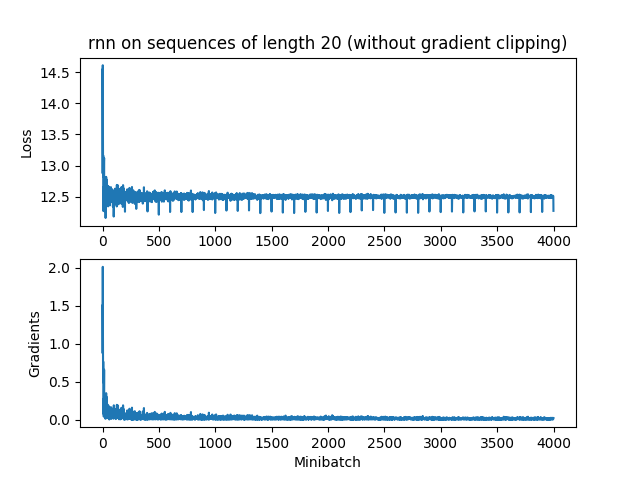
\includegraphics[scale=0.9]{q3-noclip-rnn.png}
	\label{figure:RNN no clip}
	%\caption{RNN no clip}
\end{figure}
\begin{figure}[!htbp]\centering
	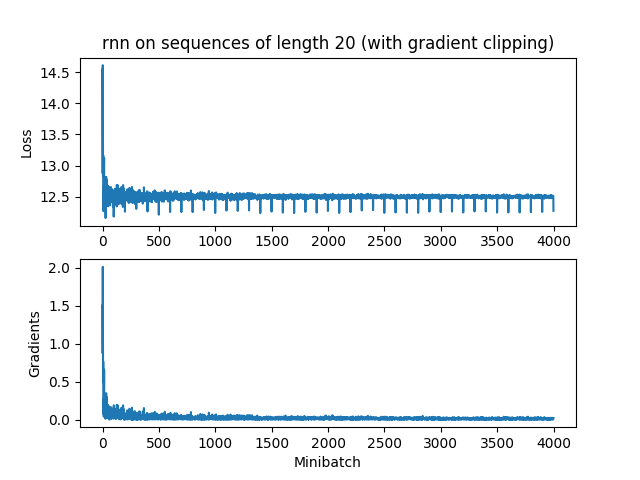
\includegraphics[scale=0.9]{q3-clip-rnn.png}
	\label{figure:RNN with clip}
	%\caption{RNN no clip}
\end{figure}
\newpage
\begin{figure}[!htbp]\centering
	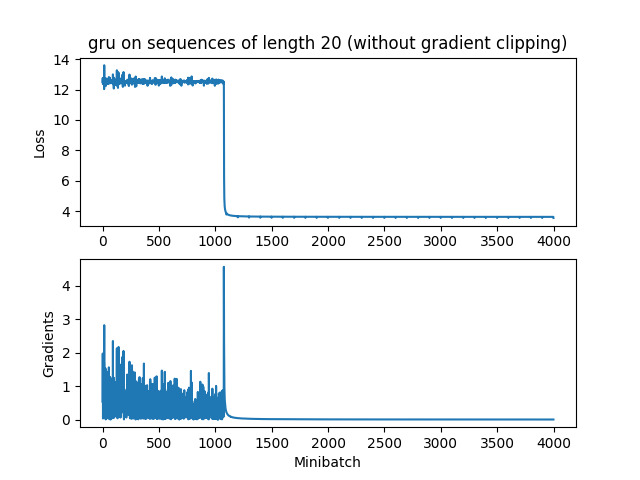
\includegraphics[scale=0.9]{q3-noclip-gru.png}
	\label{figure:GRU no clip}
	%\caption{RNN no clip}
\end{figure}
\begin{figure}[!htbp]\centering
	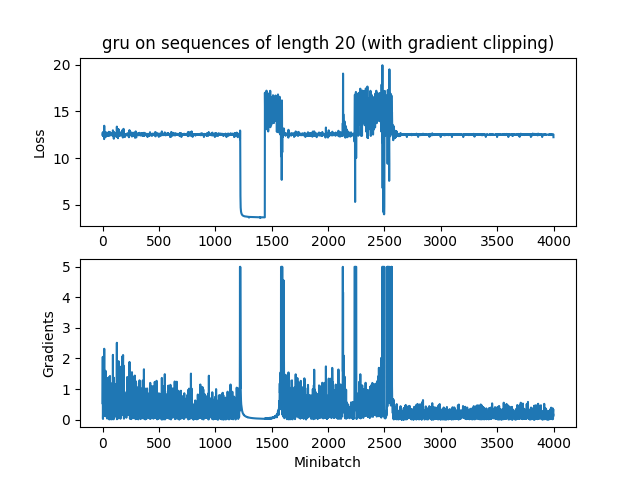
\includegraphics[scale=0.9]{q3-clip-gru.png}
	\label{figure:GRU with clip}
	%\caption{RNN no clip}
\end{figure}
\newpage
%----------------------

\subproblem{e}{Analyze graphs (5 points, written)}
\noindent \textbf{Answer:}  \\
\indent It's fine if GRU gradients are still below 5.0 without gradient clipping; just make conclusions based on what you see in your graphs. A few things to consider:

- Are gradients increasing or decreasing for the GRU with and without gradient-clipping? Is this expected?

- Does loss improve or stay constant for the RNN vs. GRU? Does gradient-clipping affect the loss? Why might this be the case?
\vskip4em
%----------------------
\subproblem{f}{Train GRU (3 points, code)}
\noindent \textbf{Answer:}  See file: $\sim$\verb|/gru_predictions.conll|.
\end{document}
